% Created 2022-09-20 Tue 09:13
% Intended LaTeX compiler: pdflatex
\documentclass[11pt]{article}
\usepackage[utf8]{inputenc}
\usepackage[T1]{fontenc}
\usepackage{graphicx}
\usepackage{longtable}
\usepackage{wrapfig}
\usepackage{rotating}
\usepackage[normalem]{ulem}
\usepackage{amsmath}
\usepackage{amssymb}
\usepackage{capt-of}
\usepackage{hyperref}
\documentclass[10pt, twoside, a4paper]{article}
\usepackage[landscape, fleqn]{geometry}
\usepackage{blindtext, fancyhdr}
\usepackage{kotex}
\usepackage{lmodern}
\usepackage[utf8]{inputenc}
\usepackage{graphicx}
\usepackage{amsmath, amsthm, amssymb}
\usepackage[table, xcdraw]{xcolor}
\usepackage{listings}
\author{syryu}
\date{\today}
\title{}
\hypersetup{
 pdfauthor={syryu},
 pdftitle={},
 pdfkeywords={},
 pdfsubject={},
 pdfcreator={Emacs 28.1 (Org mode 9.5.2)},
 pdflang={English}}
\begin{document}

\tableofcontents


\section{nix- (nix original command)}
\label{sec:orga15167d}
\begin{center}
\begin{tabular}{ll}
\$nix-env --list-generations & \$nix-env -G 42  or \$nix-env --switch-generation 42\\
\$nix-env --rollback & \\
\$nix-env -e firefox & \$nix-env -e '.*'\\
\$nix-store --delete & \$nix-store --gc\\
\$nix-collect-garbage -d & \\
\end{tabular}
\end{center}
\section{nix (nix command improved)}
\label{sec:orgfdd8c50}
\begin{center}
\begin{tabular}{ll}
\$nix-env 대응 & nix profile\\
\end{tabular}
\end{center}

\begin{center}
\begin{tabular}{lll}
\$nix-env -iA firefox & \$nix profile install firefox & \$nix profile install nixpkgs\#hello\\
\$nix-env -e firefox & \$nix profile remove firefox & \\
\$nix-env -q & \$nix profile list & \\
\$nix-env --list-generations & \$nix profile history & \\
\$nix-env --rollback & \$nix profile rollback & \\
\$nix-env -qa &  & \\
\$nix-env -qaPs &  & \\
\end{tabular}
\end{center}

\begin{center}
\begin{tabular}{lll}
\$nix profile install & \$nix profile remove & \$nix profile rollback\\
\$nix profile list & \$nix profile history & \\
\end{tabular}
\end{center}
nix-env로 설치한 App의 profile은  manifest.nix 파일로 관리되지만, nix profile 로 설치한 App은 manifest.json으로 관리된다.
nix profile로 App을 설치하면 profile의 관리 파일 자체가 바뀌기 때문에 더 이상 nix-env로 설치할 수 없다.

\begin{center}
\begin{tabular}{l}
\$nix-store -q --tree `realpath ./result/bin/S4\\
\$nix-store -q --referrers-closure `realpath ./result/bin/S4\\
\end{tabular}
\end{center}

\section{nixos}
\label{sec:org1163214}
\begin{center}
\begin{tabular}{l}
\$nixos-rebuild switch --rollback\\
[flake.nix가 있는 폴더]\$sudo nixos-rebuild switch --flake .\#syryuhds --impure\\
\end{tabular}
\end{center}

\section{flake}
\label{sec:orgf766c02}
\begin{center}
\begin{tabular}{ll}
[flake.nix가 있는 폴더]\$nix build & nix build  github:syryuauros/myflakes/master\\
[flake.nix가 있는 폴더]\$nix run & nix run  github:syryuauros/myflakes/master\\
\$ nix run nixpkgs\#gnuplot\\
\end{tabular}
\end{center}

\begin{center}
\begin{tabular}{ll}
\$realpath ./result/bin/S4 & \$nix-store -q --tree `realpath ./result/bin/S4`\\
\end{tabular}
\end{center}

\begin{center}
\begin{tabular}{l}
\$nix flake metadata github:edolstra/dwarffs\\
\end{tabular}
\end{center}

\begin{center}
\begin{tabular}{l}
\$nix flake show github:edolstra/dwarffs\\
\end{tabular}
\end{center}

\begin{center}
\begin{tabular}{l}
\$nix-store -q --referrers-closure `realpath ./result/bin/S4\\
\end{tabular}
\end{center}

\begin{center}
\begin{tabular}{l}
\$ nix registry add nixpkgs github:NixOS/nixpkgs/5272327b81ed355bbed5659b8d303cf2979b6953\\
\end{tabular}
\end{center}

\begin{center}
\begin{tabular}{l}
\$nix-info -m\\
\end{tabular}
\end{center}

\begin{center}
\begin{tabular}{l}
``\url{https://github.com/}<owner>/<project>/commit/<hash>''\\
example & \url{https://github.com/nixos/nixpkgs/commit/ede02b4ccb13557b95058d66146640a2b0bb198f}\\
\end{tabular}
\end{center}

\begin{center}
\begin{tabular}{ll}
\$nix build   (default package만 설치) & \$nix build .\#s4 .\#gnuplot (default외에 다른 package설치를 위해서는 직접 package명을 입력해야 한다.)\\
\end{tabular}
\end{center}

\subsection{flake override}
\label{sec:org5f78446}
\begin{center}
\begin{tabular}{l}
ex) (openblas.override \{ singleThreaded = true;\})\\
\end{tabular}
\end{center}

\begin{center}
\begin{tabular}{l}
or let openblas-single-thread = openblas.override \{ singleThreaded = true; \};\\
\end{tabular}
\end{center}
\section{nix-shell}
\label{sec:orge46b55f}
\begin{center}
\begin{tabular}{l}
nix-shell -p 'lua.withPackages(ps: with ps; [ busted luafilesystem ])'\\
\end{tabular}
\end{center}

\section{nixpkgs}
\label{sec:orgae3866e}
\subsection{confirm packages for nix-build, nix-instantiate, nix-channel}
\label{sec:orgdb9cc98}
\begin{center}
\begin{tabular}{rl}
1 & \$nixrepl [Ret] nix-repl>:l <nixpkgs> [Ret] nix-repl>keyword(ex:rust) + TAB\\
2 & /nix/var/nix/profiles/per-user/root/channels/nixos/pkgs/top-level/all-packages.nix\\
3 & \$cd `nix-instantiate --eval -E '<nixpkgs>'` [Ret] cat > all-packages.nix\\
4 & \$NIX\_PATH, 경로 확인 후 이동해서 all-packages.nix 확인\\
\end{tabular}
\end{center}

\subsection{confirm packages for nix-env}
\label{sec:org249ec8a}
\begin{center}
\begin{tabular}{rl}
1 & \$nix-env -qa 'keyword.*' or \$nix-env -qaPs 'keyword'\\
2 & \$cd \textasciitilde{}/.nix-defexpr/channels\_root/nixos/pkgs/top-level, all-packages.nix\\
\end{tabular}
\end{center}

\subsection{confirm packages for flakes}
\label{sec:orgf20e188}
\begin{center}
\begin{tabular}{rl}
1 & flake.lock 파일 확인 >> ``nixpkgs'' 항목의 ``rev'' term 확인 >> github.com/[owner]/[repo]/tree/[rev]\\
\end{tabular}
\end{center}
그림 참조

\section{nix repl}
\label{sec:org56a36a6}
\subsection{nix-repl> 명령어}
\label{sec:orge10bf35}
\begin{center}
\begin{tabular}{ll}
:help & 도움말\\
입력 중간에 TAB & 자동 완성\\
:doc keyword & 해당 명령어 도움말\\
 & \\
\end{tabular}
\end{center}

\section{pictures}
\label{sec:org205f0e9}
\begin{center}
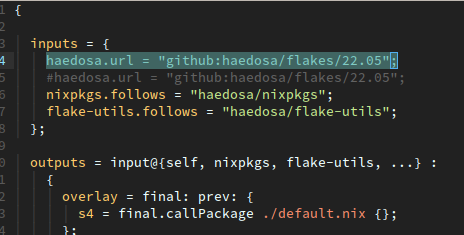
\includegraphics[width=.9\linewidth]{./img/3_nix/flake input url.png}
\label{flake input url}
\end{center}

\begin{center}
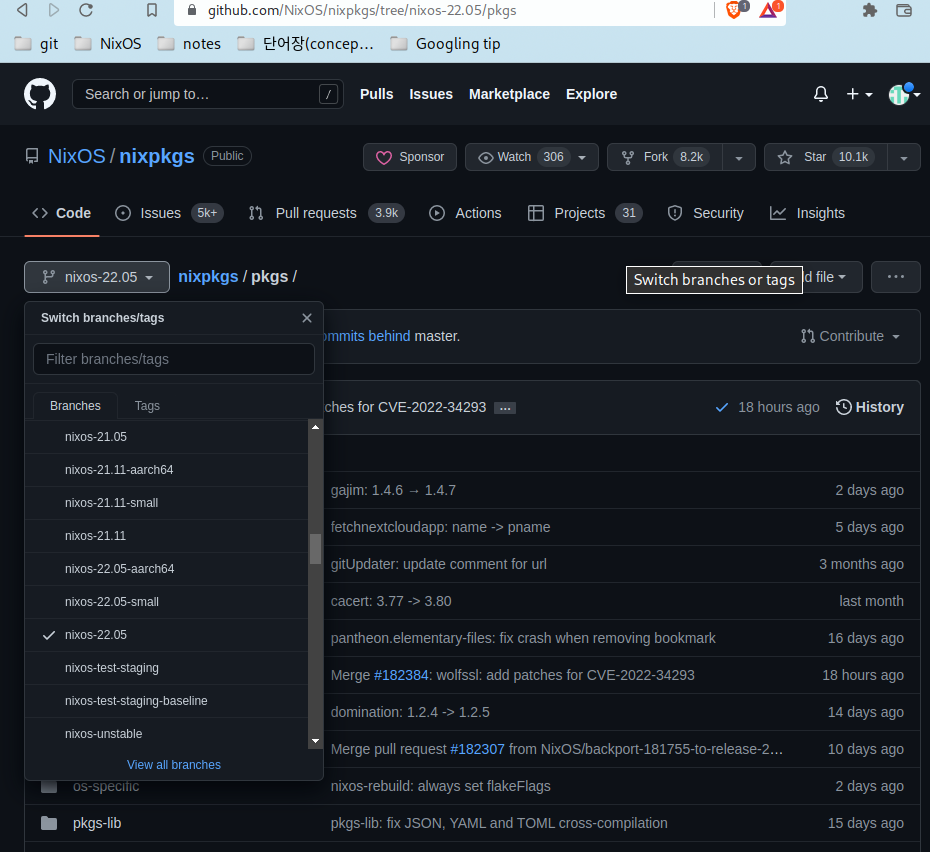
\includegraphics[width=.9\linewidth]{./img/3_nix/real repo flake indicate.png}
\end{center}
\begin{center}
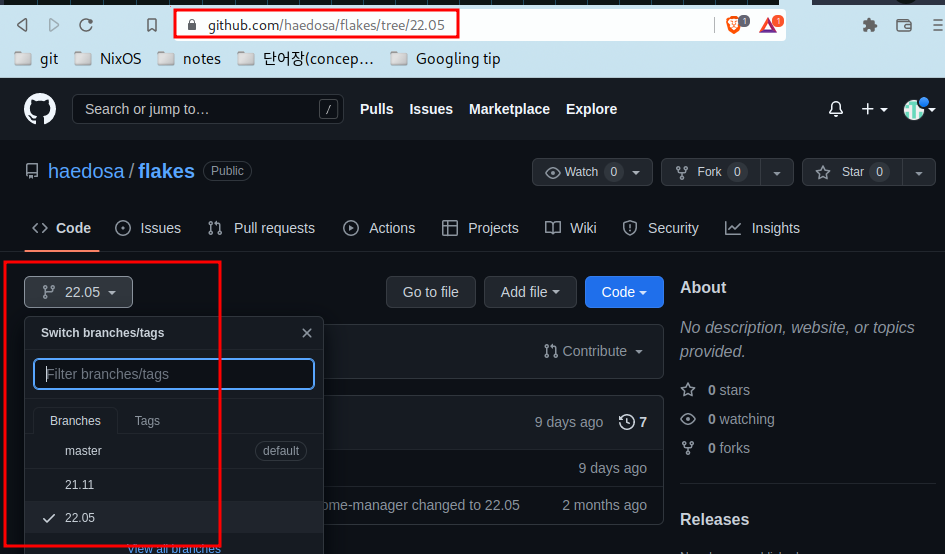
\includegraphics[width=.9\linewidth]{./img/3_nix/real repo flake indicate_2.png}
\end{center}
\begin{center}
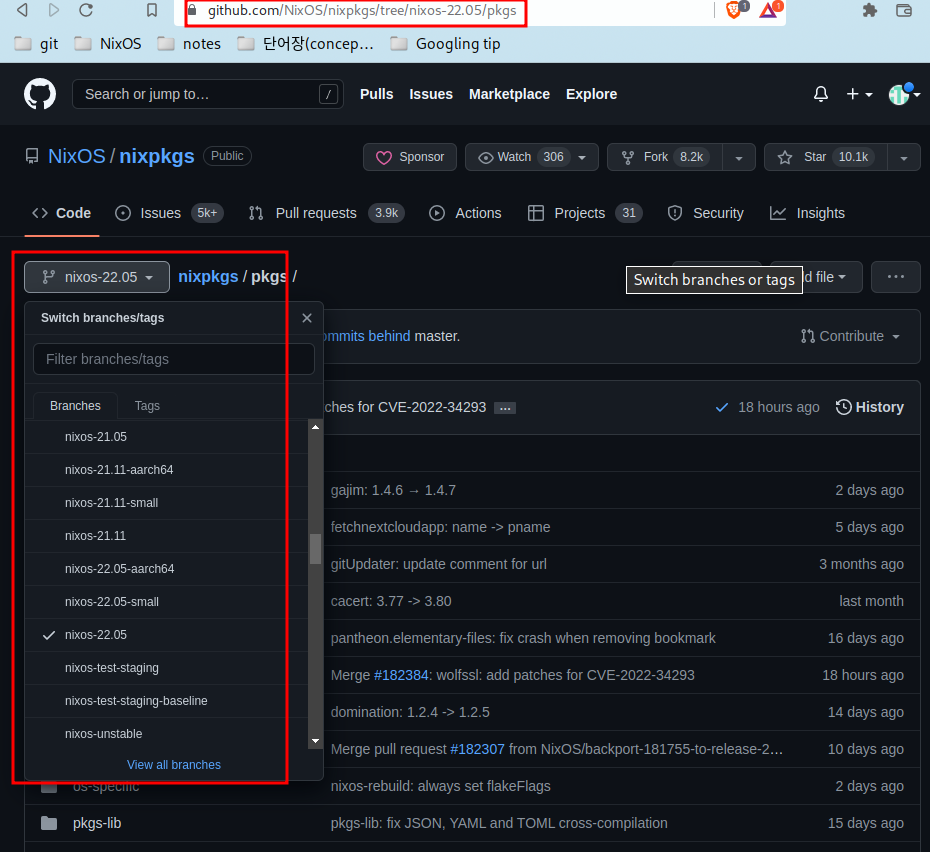
\includegraphics[width=.9\linewidth]{./img/3_nix/real repo flake indicate_3.png}
\end{center}

\begin{center}
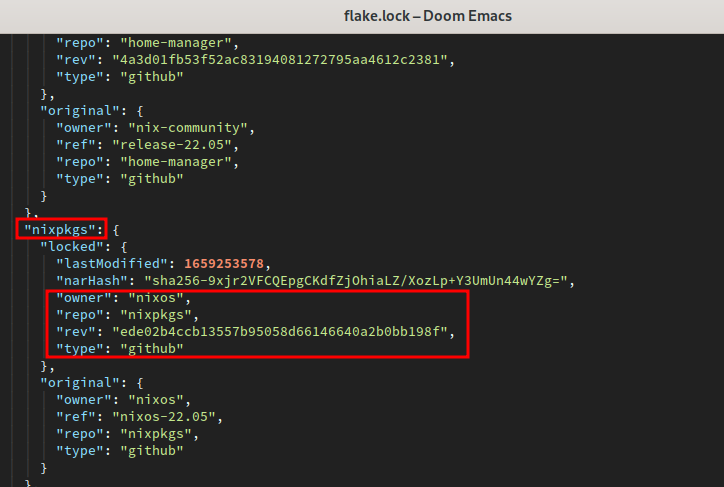
\includegraphics[width=.9\linewidth]{./img/3_nix/repo find from flake.lock.png}
\end{center}
\begin{center}
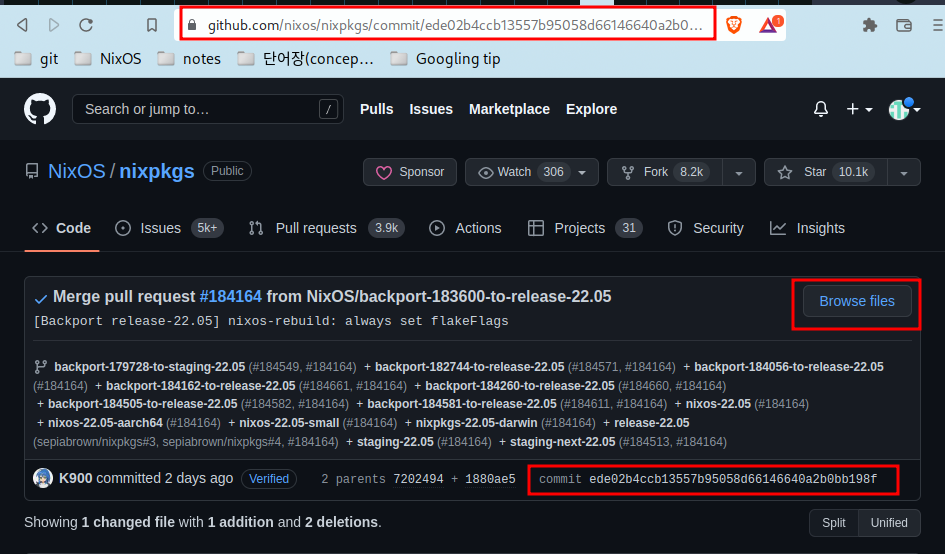
\includegraphics[width=.9\linewidth]{./img/3_nix/repo find from flake.lock2.png}
\end{center}
\begin{center}
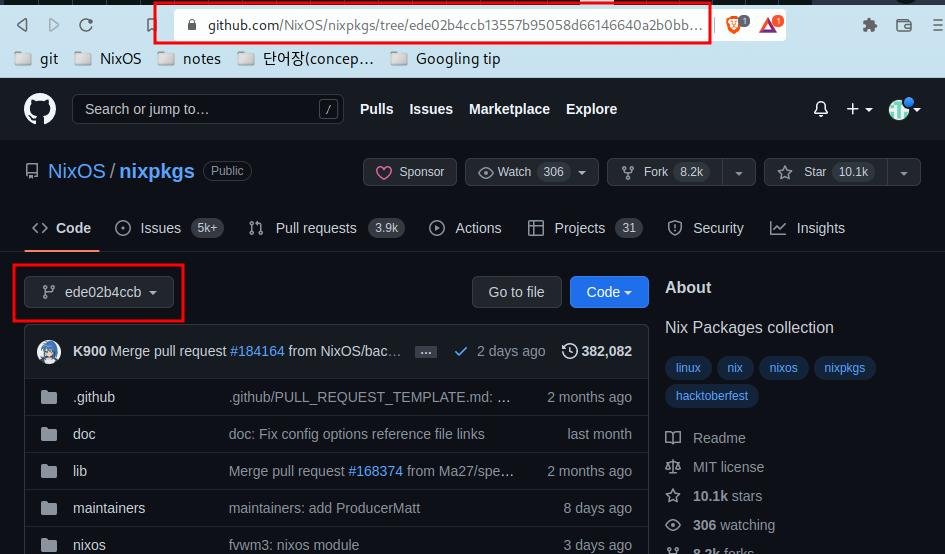
\includegraphics[width=.9\linewidth]{./img/3_nix/repo find from flake.lock3.png}
\end{center}

\begin{center}
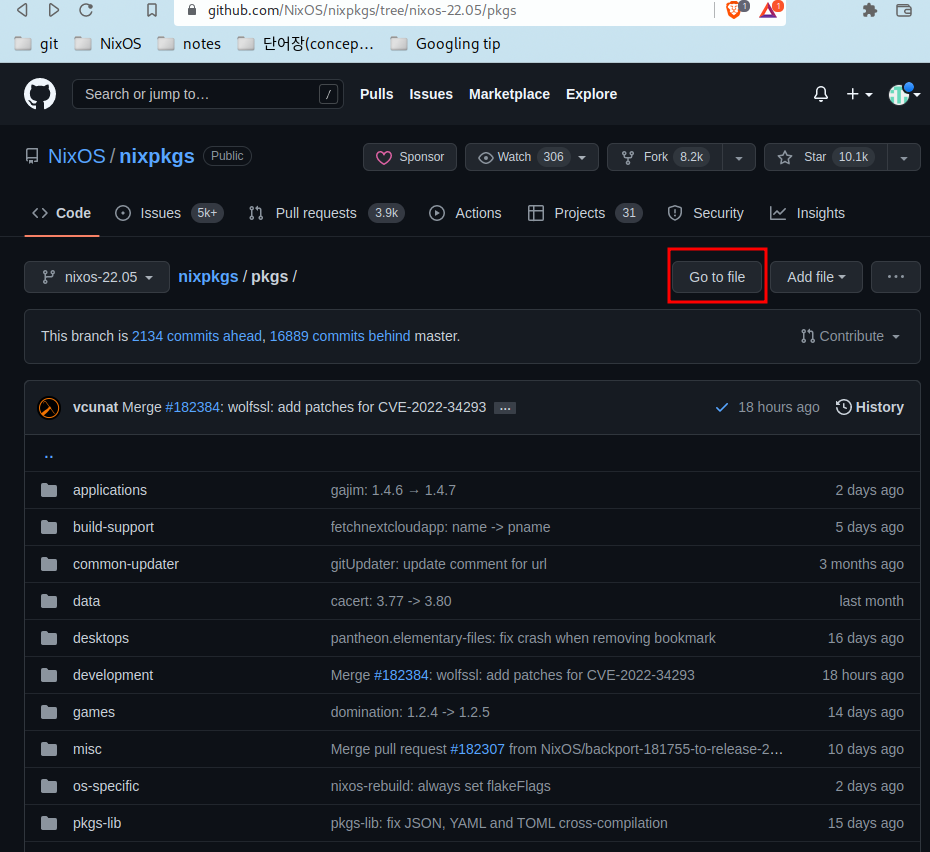
\includegraphics[width=.9\linewidth]{./img/3_nix/how to find packages_1.png}
\end{center}
\begin{center}
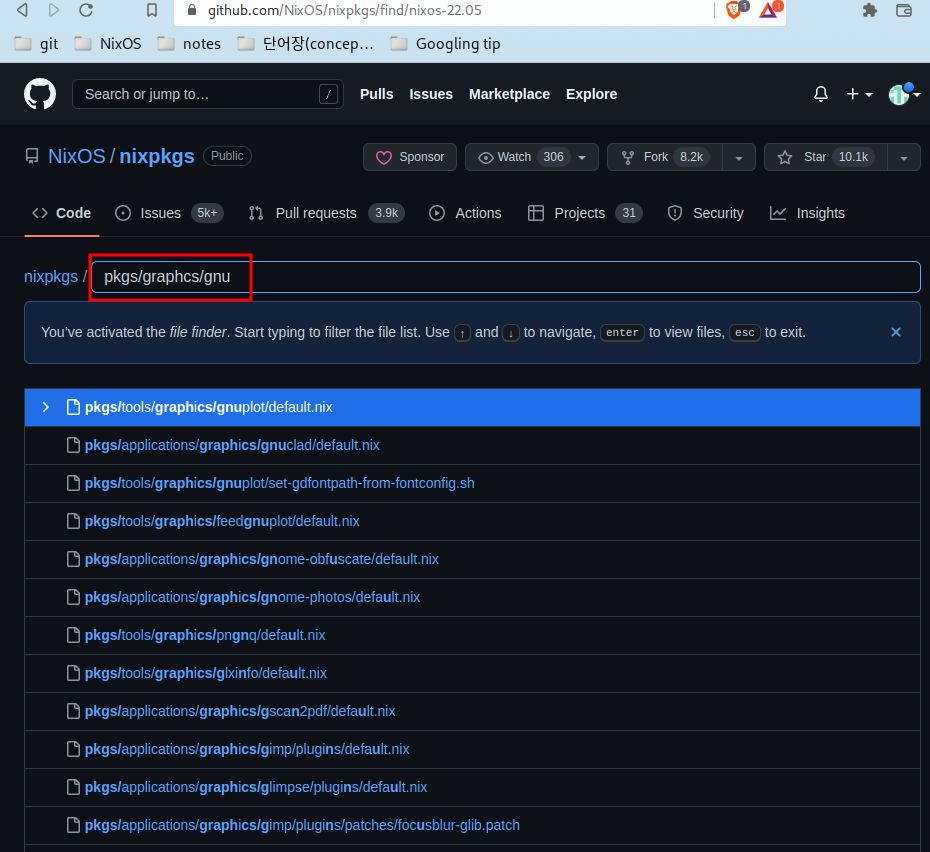
\includegraphics[width=.9\linewidth]{./img/3_nix/how to find packages_2.png}
\end{center}
.
\end{document}
